\documentclass[tikz,border=8pt]{standalone}
\usepackage{amsmath,amssymb}
\usepackage{tikz}
\usetikzlibrary{positioning,fit,backgrounds,calc}

\tikzset{
  obs/.style={circle, draw=black, thick, minimum size=9mm, inner sep=0pt},
  latent/.style={circle, draw=black, thick, fill=gray!18, minimum size=9mm, inner sep=0pt},
  const/.style={rectangle, draw=black, thick, minimum size=7mm, inner sep=1pt},
  factor/.style={rectangle, draw=black, thick, fill=white, minimum width=5mm, minimum height=5mm, inner sep=0pt},
  plate/.style={draw=black, rounded corners=2pt, inner sep=8pt},
}

\begin{document}
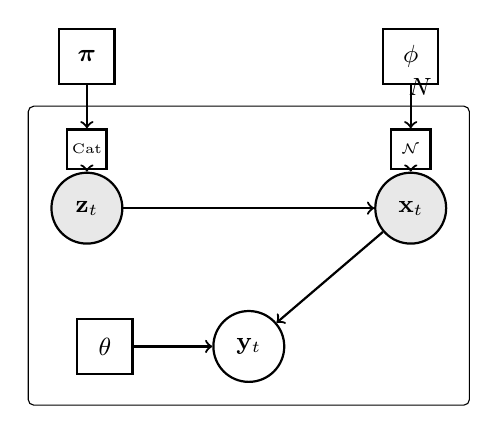
\begin{tikzpicture}[
  node distance=1.1cm and 1.4cm,
  font=\small,
  every node/.style={align=center}
]
  \node[obs] (y) {$\mathbf{y}_t$};
  \node[latent, above left=of y] (x1) {$\mathbf{z}_{t}$};
  \node[const, above=of x1] (pi) {$\boldsymbol{\pi}$};
  \node[latent, above right=of y] (x2) {$\mathbf{x}_{t}$};
  \node[const, above=of x2] (phi) {$\phi$};
  \node[const, left=1.0cm of y] (theta) {$\theta$};

  \node[factor, below=0.55cm of pi] (factoxT) {\tiny Cat};
  \node[factor, below=0.55cm of phi] (factoyT) {\tiny $\mathcal{N}$};

  \draw[->, thick] (pi) -- (factoxT);
  \draw[->, thick] (factoxT) -- (x1);
  \draw[->, thick] (phi) -- (factoyT);
  \draw[->, thick] (factoyT) -- (x2);
  \draw[->, thick] (x1) -- (x2);
  \draw[->, thick] (x2) -- (y);
  \draw[->, thick] (theta) -- (y);

  \begin{scope}[on background layer]
    \node[plate, fit=(x1)(x2)(y)(factoxT)(factoyT), label=above right:{$N$}] (plate1) {};
  \end{scope}
\end{tikzpicture}
\end{document}
